\begingroup \pagestyle{empty}

\begin{titlepage} \thispagestyle{empty} \begin{tikzpicture}[remember picture, overlay]
\node[anchor=south west, inner sep=0] at (current page.south west) {%
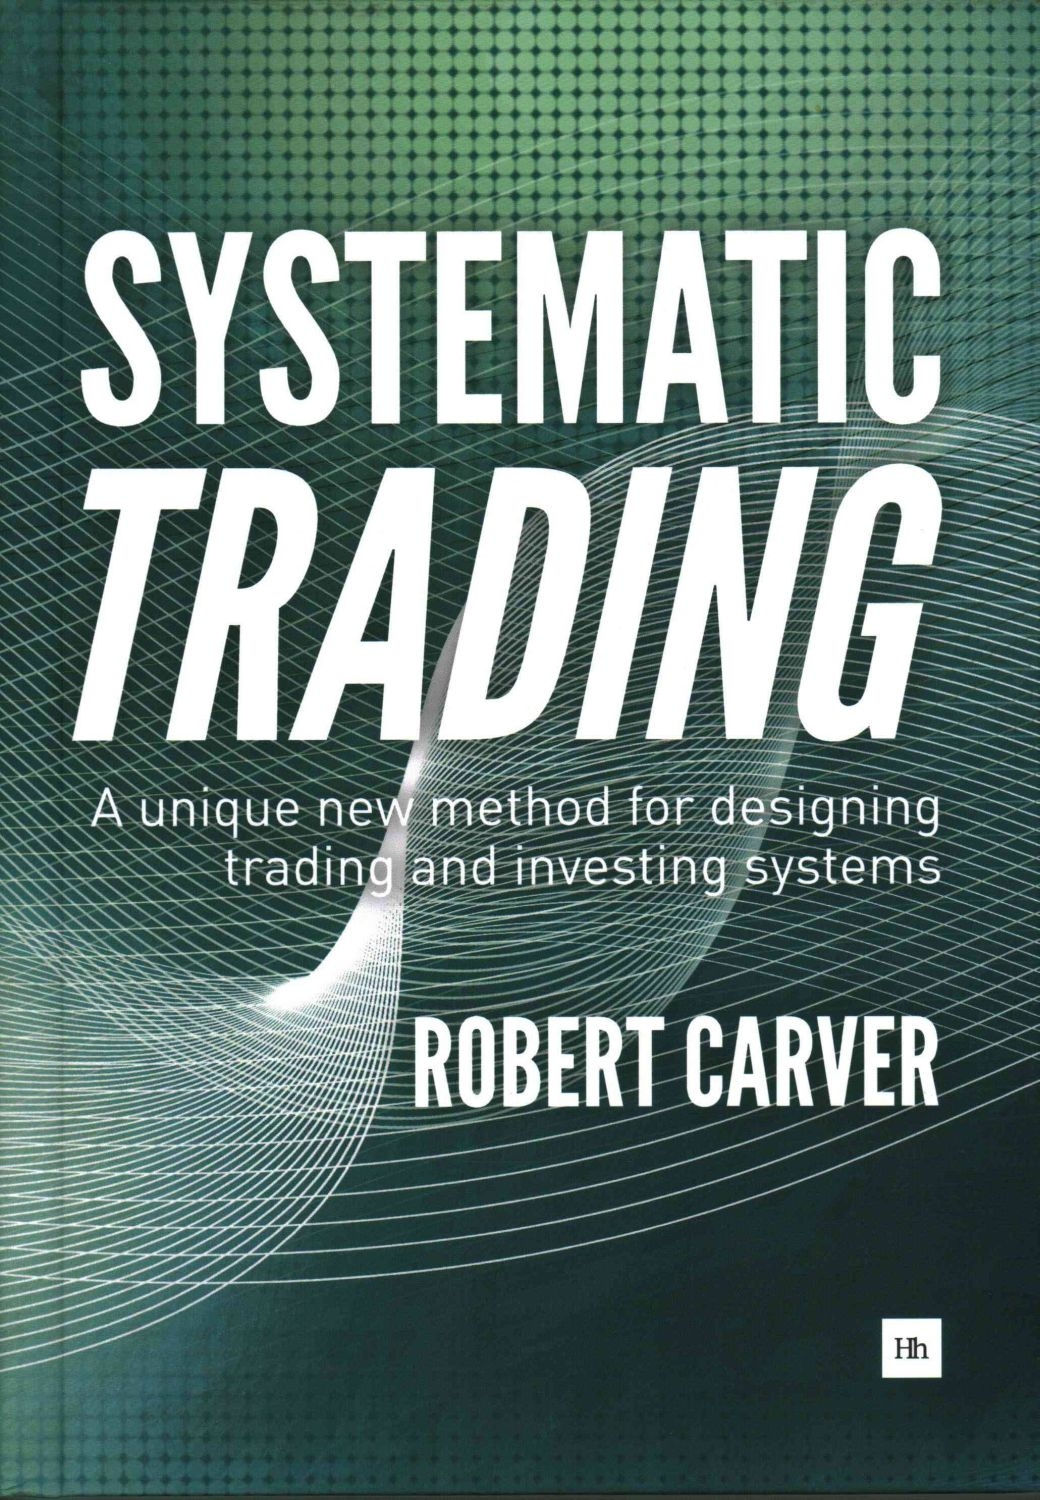
\includegraphics[width=\paperwidth,height=\paperheight]{figures/raw/img-000.jpg}%
};\end{tikzpicture}
\null \end{titlepage}

\thispagestyle{empty} \begin{center} \vspace*{0.19\textheight}
{\Huge\bfseries Systematic Trading\par}
\vspace{2.2cm} \end{center}

\begin{center} \begin{minipage}{\textwidth}
%    \centering
\small Robert Carver worked in the City of London for over a decade. He initially traded exotic derivative products for Barclays Investment Bank and then worked as a portfolio manager for AHL --- one of the world's largest systematic hedge funds --- before, during and after the global financial meltdown of 2008. He was responsible for the creation of AHL's fundamental global macro strategy and then managed the fund's multi-billion dollar fixed income portfolio before retiring from the industry in 2013. Robert, who has bachelors and masters degrees in Economics, now systematically trades his own portfolio of futures and equities. \end{minipage}
\end{center}

\clearpage \thispagestyle{empty} \begin{center} \vspace*{0.22\textheight} \begin{minipage}{0.72\textwidth} \centering \small Every owner of a physical copy of this version of\\[0.3em]
{\Large\bfseries Systematic Trading}\\[0.3em]
can download the eBook for free direct from\\
us at Harriman House, in a format that can be\\
read on any eReader, tablet or smartphone.\\[1.1em]
{\color{bookrule}\rule{0.22\textwidth}{0.8pt}}\\[1.1em]
Simply head to:\\[0.35em]
\url{ebooks.harriman-house.com/systematictrading}\\[0.35em]
to get your free eBook now. \end{minipage}
\end{center}

\clearpage \thispagestyle{empty} \begin{center} \vspace*{0.22\textheight}
{\Huge\bfseries Systematic Trading\par}
\vspace{0.8em}
{\Large\bfseries A unique new method for designing trading\\and investing systems\par}
\vspace{1.6em} {\color{bookrule}\rule{0.18\textwidth}{0.8pt} \par } \vspace{2.1cm}
{\Large Robert Carver\par}
\end{center}

\clearpage \thispagestyle{empty} \begingroup \footnotesize \setlength{\parindent}{0pt} \leftskip=0.12\textwidth \rightskip=0.12\textwidth \raggedright HARRIMAN HOUSE LTD\\
18 College Street\\
Petersfield\\
Hampshire\\
GU31 4AD\\
GREAT BRITAIN\\
Tel: +44 (0)1730 233870\\
Email: contact@harriman-house.com\\
Website: \url{www.harriman-house.com} \par

\vspace{1.1em} First published in Great Britain in 2015\\
Copyright \copyright{} Robert Carver\\
The right of Robert Carver to be identified as the Author has been asserted in accordance with the Copyright, Designs and Patents Act 1988. \par

\vspace{1.1em} Hardback ISBN: 9780857194459\\
eBook ISBN: 9780857195005 \par

\vspace{1.1em} British Library Cataloguing in Publication Data\\
A CIP catalogue record for this book can be obtained from the British Library. \par

\vspace{0.85em} All rights reserved; no part of this publication may be reproduced, stored in a retrieval system, or transmitted in any form or by any means, electronic, mechanical, photocopying, recording, or otherwise without the prior written permission of the Publisher. This book may not be lent, resold, hired out or otherwise disposed of by way of trade in any form of binding or cover other than that in which it is published, without the prior written consent of the Publisher. \par

\vspace{0.85em} No responsibility for loss occasioned to any person or corporate body acting or refraining to act as a result of reading material in this book can be accepted by the Publisher, by the Author, or by the Employer of the Author. \par

\vspace{0.85em} Page number cross references refer to the print edition. \par \endgroup \normalsize

\clearpage \thispagestyle{empty} \begin{center} \vspace*{0.29\textheight} \begin{minipage}{\textwidth} ``In every case the accuracy of experts was matched or exceeded by a simple algorithm... Why are experts inferior to algorithms? One reason... is that experts try to be clever, think outside the box, and consider complex combinations of features in making their predictions. Complexity may work in the odd case but more often than not it reduces validity.''\\[1.5em]
Daniel Kahneman, \textit{Thinking, Fast and Slow} \end{minipage}
\end{center}

\endgroup
